\chapter{関連語句}
\section{脳情報デコーディング}
脳情報デコーディングとは,脳活動を読み取る技術である.
デコーディングとは,符号列を元の状態に戻す作業を指す言葉である.
たとえば脳が外界から何らかの刺激を受け取っていた場合,脳情報デコーディング技術を用いて,その刺激について第三者が解読可能である.
脳情報デコーディングは,外界の刺激や行動,認知状態と,その時の脳活動との関連性を学習するステップと,
その学習結果をもとに脳活動から外界の刺激や行動,認知状態を予測するステップからなる.
脳情報デコーディングを用いた研究例として,運動情報の読み取りが挙げられる.
ヒト運動野のfMRI信号を用いてジャンケンを行う例では,ヒトが「チョキ」を出したときの脳活動を計測し,脳活動パターン解析結果により,限りなくリアルタイムに近い状態でロボットに実験参加者と同じジャンケンをさせることができる.
今回の課題では,第\ref{chap:\kadaie}章の\kadaie が脳情報デコーディングにあたる.\\
\hfill\cite{脳情報デコーディング技術とその応用}
\section{視線入力インタフェース}
視線入力インタフェースとは,視線により,利用者の意思を入力するシステムであり,肢体障がい者のコミュニケーション手段として研究されてきた.
視線入力システムには,いくつか方法があるが,ここでは大きく「眼球運動測定法」を取り上げ,
眼球運動測定法はさらに,眼電図法(EOG),強膜反射法,角膜反射法,瞳孔\ -\ 角膜反射法に分けられている.
ここでは角膜反射法について取り上げよう.角膜反射法とは,角膜上に光の反射点を生じさせ,眼球の画像を撮影した後,
撮影した眼球の画像から,角膜上の光の反射点と瞳孔を識別する.この結果により眼球の方向を算出する.
この技術は,第\ref{chap:\kadaia}章の\elt ,第\ref{chap:\kadaid}章の\tobi に用いられている技術である.\\
\hfill\cite{weko_847_1}

\begin{wrapfigure}{r}[0mm]{.4\textwidth}
    \centering
    \begin{minipage}{.19\textwidth}
        \centering
        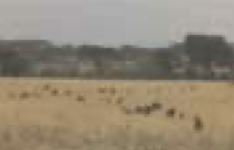
\includegraphics[height=2cm,width=\textwidth]{../../Figures/kenty2.png}
        \subcaption{入力画像}
    \end{minipage}
    \begin{minipage}{.19\textwidth}
        \centering
        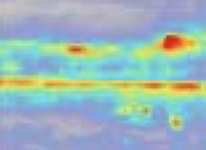
\includegraphics[height=2cm,width=\textwidth]{../../Figures/kenty1.png}
        \subcaption{顕著性マップ}
    \end{minipage}
    \caption{顕著性マップの例\cite{動画像コンテンツにおける注視点マップと顕著性マップとの関係性に関する考察}}
    \vspace{-1.3cm}
\end{wrapfigure}
\section{顕著性マップ}
\begin{quote}
    ``顕著性マップとは,人が画像を認識する際に注視しやすい部分を画像で表現したものである.''\hfill\cite{顕著性マップを用いた画質評価法}
\end{quote}
第\ref{chap:\kadaib}章の\figref{fig:実験結果\kadaid}で示しているHeat Mapは,「刺激画像のどこをより注視しているか」を色で表現したものであった.
\figref{fig:実験結果\kadaid}は単なる結果であるが,顕著性マップは画像の物理的特徴を解析して注意が向けられる位置を推定する.
大まかな処理を説明する.まず入力画像に対して,6つの特徴マップ(色,彩度,方位,コントラスト,点滅,運動)を作成する.
特徴マップ合成では,6つの生成した特徴マップを線形和し,顕著性マップを算出する.
顕著性マップを用いることで,実験による注視箇所の特定をせずとも,刺激に対する注視箇所がわかるため,
テレビ放送などのコマーシャル,包装容姿のデザインなど,商用利用も多く,我々との生活で密にかかわっている.\\
\hfill\cite{動画像コンテンツにおける注視点マップと顕著性マップとの関係性に関する考察}
\section{分散分析}
第\ref{chap:\kadaia}章で\(t\)検定を用いて2正規母集団の「回帰直線傾きの平均」が異なるか否かを検証した.
ここで,3つ以上の正規母集団の母平均が異なるか否かを検証する.
このとき,\(t\)検定を3回行う方法では正しい結果を導けない.
ここで用いられるのが分散分析(analysis of variance: ANOVA)である.
検定の対象は,母分散ではなく母平均だが,母平均の差を検定するために母分散を利用することが,この名前の由来である.
分散分析には主に,「一元配置分散分析」と「二元配置分散分析」の2種類がある.
一元配置分散分析は,母平均の差を生む要因が1つの場合に用い,二元配置分散分析は,母平均の差を生む要因が2つの場合に用いる.\\
\hfill\cite[p.170,\ p.179]{Rで学ぶ統計データ分析}